\documentclass[a4paper]{article}

% Set page size and margins
% Replace `letterpaper' with `a4paper' for UK/EU standard size
\usepackage[letterpaper,top=2cm,bottom=2cm,left=2.5cm,right=2.5cm,marginparwidth=1.75cm]{geometry}

\usepackage[ruled, linesnumbered]{algorithm2e}
\SetKwProg{Fn}{Function}{}{end}

% Useful packages
\usepackage{amsmath,amssymb}
\usepackage{graphicx}
\usepackage[colorlinks=true, allcolors=blue]{hyperref}
\usepackage{multicol}
\usepackage{url}

% Chinese Support
\usepackage[CJKmath=true,AutoFakeBold=3,AutoFakeSlant=.2]{xeCJK}   
\setCJKmainfont{NOTOSERIFTC-MEDIUM.OTF}
%\setCJKmainfont{fonts/NOTOSERIFTC-MEDIUM.OTF}

\usepackage{amsfonts}
\usepackage{mathtools}
\newcommand{\defeq}{\vcentcolon=}
\newcommand{\eqdef}{=\vcentcolon}

\usepackage{framed}
\usepackage{graphicx}

% Figures
\newenvironment{Figure}
  {\par\medskip\noindent\minipage{\linewidth}}
  {\endminipage\par\medskip}
\usepackage{caption}
\usepackage{wrapfig}
\usepackage{wrapfig}
\usepackage{graphicx}
\usepackage[export]{adjustbox}
\usepackage{subcaption}

\setlength\parindent{0pt}
\linespread{1.25}


\graphicspath{../imgaes}
% \newcommand{\twocolimg}[4]{\begin{figure}[!ht]
%     \centering
%     \begin{subfigure}[t]{.4\textwidth}
%     \centering
%     \includegraphics[width=0.9\linewidth]{#2}
%     \caption{#1}
%     \end{subfigure}
%     \begin{subfigure}[t]{.4\textwidth}
%     \centering
%     \includegraphics[width=0.9\linewidth]{#4}
%     \caption{#3}
%     \end{subfigure}
% \end{figure}}

\usepackage{wrapfig}

\usepackage{listings}
\lstset{basicstyle=\ttfamily,
  showstringspaces=false,
  commentstyle=\color{red},
  keywordstyle=\color{blue},
  language=Python
}

% \theoremstyle{definition}
% \newtheorem*{definition}{Definition}

% \newtheorem*{theorem*}{Theorem}
% \newtheorem*{lemma}{Lemma}


\title{DIP Final Report}


\begin{document}
\SetKwProg{Fn}{Function}{}{end}
\maketitle


\newpage
\begin{figure}
  \begin{subfigure}{0.9\textwidth}
   \centering
\begin{subfigure}[t]{0.22\textwidth}
    \includegraphics[width=0.9\linewidth]{../images/outputs/erosion\_exp/lena\_erosion1.png}
    
    \centering
  \end{subfigure}
\begin{subfigure}[t]{0.22\textwidth}
    \includegraphics[width=0.9\linewidth]{../images/outputs/erosion\_exp/lena\_erosion3.png}
    
    \centering
  \end{subfigure}
\begin{subfigure}[t]{0.22\textwidth}
    \includegraphics[width=0.9\linewidth]{../images/outputs/erosion\_exp/lena\_erosion5.png}
    
    \centering
  \end{subfigure}
 \caption{erosion with different SE}
 \end{subfigure}

\end{figure}

\begin{figure}[!ht]
   \centering
\begin{subfigure}[t]{0.25\textwidth}
    \includegraphics[width=0.9\linewidth]{../images/outputs/noise\_exp/lena\_salt.png}
    \caption{salt noise}
    \centering
  \end{subfigure}
\begin{subfigure}[t]{0.25\textwidth}
    \includegraphics[width=0.9\linewidth]{../images/outputs/noise\_exp/lena\_salt\_opening.png}
    \caption{salt noise opening}
    \centering
  \end{subfigure}
\begin{subfigure}[t]{0.25\textwidth}
    \includegraphics[width=0.9\linewidth]{../images/outputs/noise\_exp/lena\_salt\_closing.png}
    \caption{salt noise closing}
    \centering
  \end{subfigure}
\begin{subfigure}[t]{0.25\textwidth}
    \includegraphics[width=0.9\linewidth]{../images/outputs/noise\_exp/lena\_pepper.png}
    \caption{pepper noise}
    \centering
  \end{subfigure}
\begin{subfigure}[t]{0.25\textwidth}
    \includegraphics[width=0.9\linewidth]{../images/outputs/noise\_exp/lena\_pepper\_opening.png}
    \caption{pepper noise opening}
    \centering
  \end{subfigure}
\begin{subfigure}[t]{0.25\textwidth}
    \includegraphics[width=0.9\linewidth]{../images/outputs/noise\_exp/lena\_pepper\_closing.png}
    \caption{pepper noise closing}
    \centering
  \end{subfigure}
 \caption{pepper/salt noise}
 \end{figure}


\begin{figure}
  \centering
  \begin{subfigure}{0.9\textwidth}
   \centering
\begin{subfigure}[t]{0.15\textwidth}
    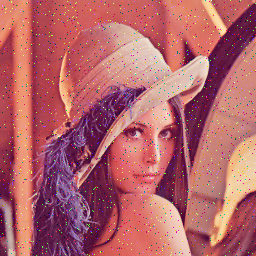
\includegraphics[width=0.9\linewidth]{../images/outputs/denoise/before/before0.png}
    
    \centering
  \end{subfigure}
\begin{subfigure}[t]{0.15\textwidth}
    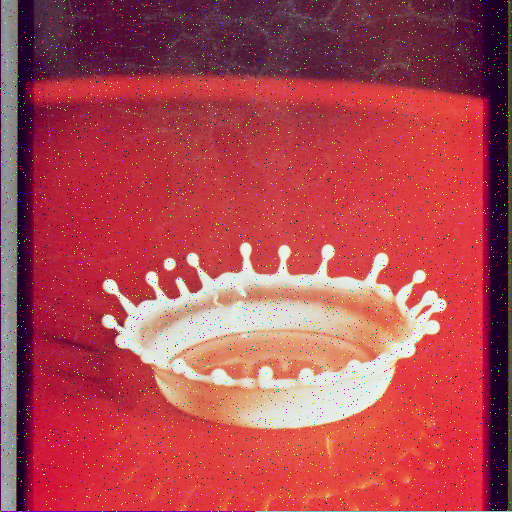
\includegraphics[width=0.9\linewidth]{../images/outputs/denoise/before/before1.png}
    
    \centering
  \end{subfigure}
\begin{subfigure}[t]{0.15\textwidth}
    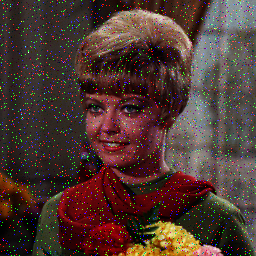
\includegraphics[width=0.9\linewidth]{../images/outputs/denoise/before/before2.png}
    
    \centering
  \end{subfigure}
\begin{subfigure}[t]{0.15\textwidth}
    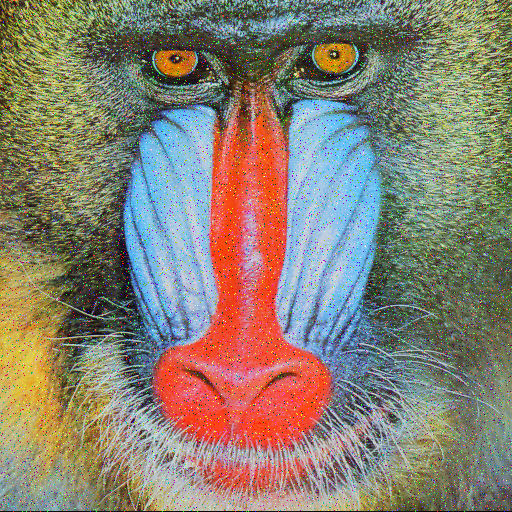
\includegraphics[width=0.9\linewidth]{../images/outputs/denoise/before/before3.png}
    
    \centering
  \end{subfigure}
\begin{subfigure}[t]{0.15\textwidth}
    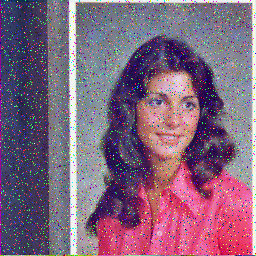
\includegraphics[width=0.9\linewidth]{../images/outputs/denoise/before/before4.png}
    
    \centering
  \end{subfigure}
\begin{subfigure}[t]{0.15\textwidth}
    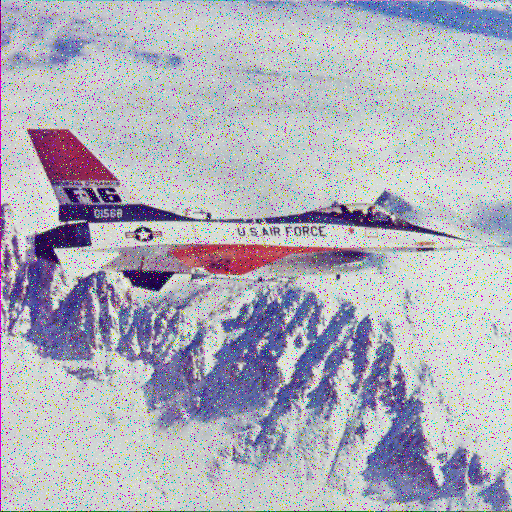
\includegraphics[width=0.9\linewidth]{../images/outputs/denoise/before/before5.png}
    
    \centering
  \end{subfigure}
 \caption{Noisy images}
 \end{subfigure}

  \begin{subfigure}{0.9\textwidth}
   \centering
\begin{subfigure}[t]{0.15\textwidth}
    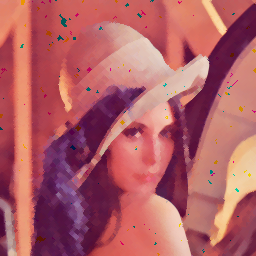
\includegraphics[width=0.9\linewidth]{../images/outputs/denoise/oc/oc0.png}
    
    \centering
  \end{subfigure}
\begin{subfigure}[t]{0.15\textwidth}
    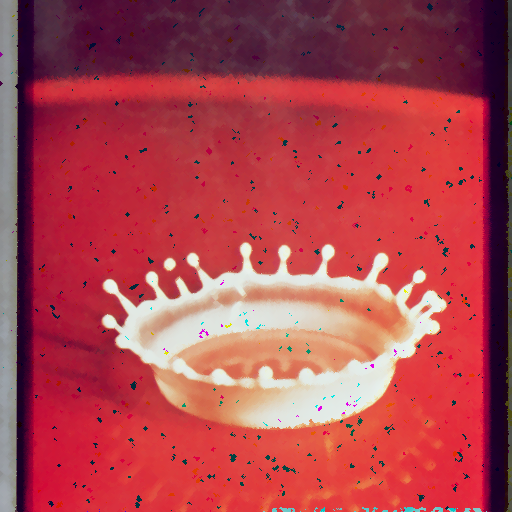
\includegraphics[width=0.9\linewidth]{../images/outputs/denoise/oc/oc1.png}
    
    \centering
  \end{subfigure}
\begin{subfigure}[t]{0.15\textwidth}
    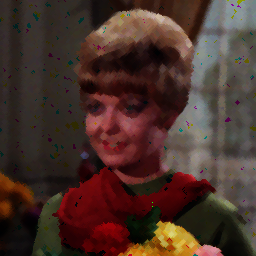
\includegraphics[width=0.9\linewidth]{../images/outputs/denoise/oc/oc2.png}
    
    \centering
  \end{subfigure}
\begin{subfigure}[t]{0.15\textwidth}
    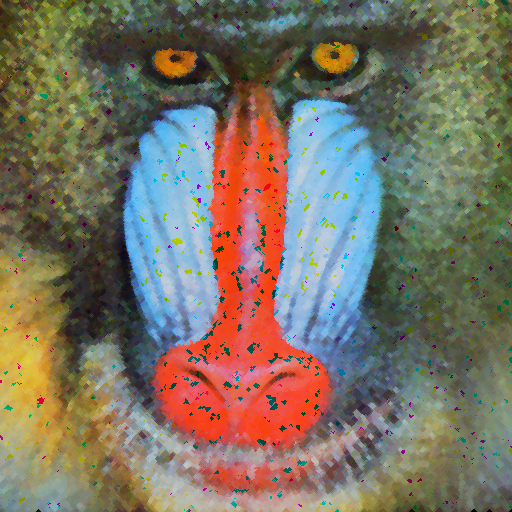
\includegraphics[width=0.9\linewidth]{../images/outputs/denoise/oc/oc3.png}
    
    \centering
  \end{subfigure}
\begin{subfigure}[t]{0.15\textwidth}
    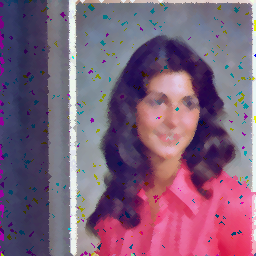
\includegraphics[width=0.9\linewidth]{../images/outputs/denoise/oc/oc4.png}
    
    \centering
  \end{subfigure}
\begin{subfigure}[t]{0.15\textwidth}
    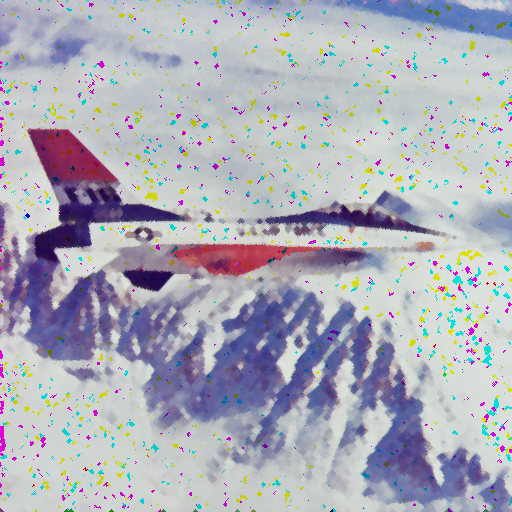
\includegraphics[width=0.9\linewidth]{../images/outputs/denoise/oc/oc5.png}
    
    \centering
  \end{subfigure}
 \caption{open-closing with proposed method}
 \end{subfigure}

  \begin{subfigure}{0.9\textwidth}
   \centering
\begin{subfigure}[t]{0.15\textwidth}
    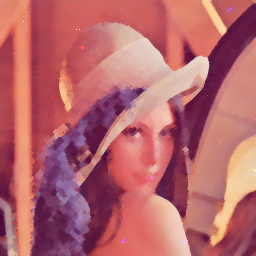
\includegraphics[width=0.9\linewidth]{../images/outputs/denoise/co/co0.png}
    
    \centering
  \end{subfigure}
\begin{subfigure}[t]{0.15\textwidth}
    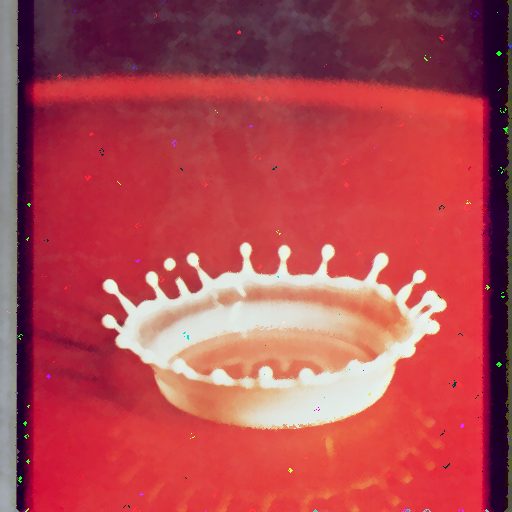
\includegraphics[width=0.9\linewidth]{../images/outputs/denoise/co/co1.png}
    
    \centering
  \end{subfigure}
\begin{subfigure}[t]{0.15\textwidth}
    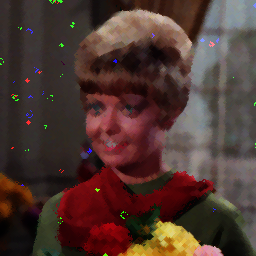
\includegraphics[width=0.9\linewidth]{../images/outputs/denoise/co/co2.png}
    
    \centering
  \end{subfigure}
\begin{subfigure}[t]{0.15\textwidth}
    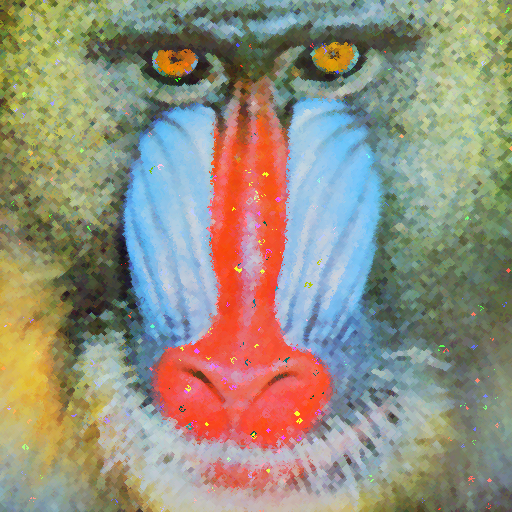
\includegraphics[width=0.9\linewidth]{../images/outputs/denoise/co/co3.png}
    
    \centering
  \end{subfigure}
\begin{subfigure}[t]{0.15\textwidth}
    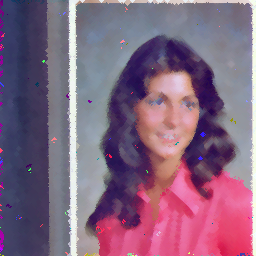
\includegraphics[width=0.9\linewidth]{../images/outputs/denoise/co/co4.png}
    
    \centering
  \end{subfigure}
\begin{subfigure}[t]{0.15\textwidth}
    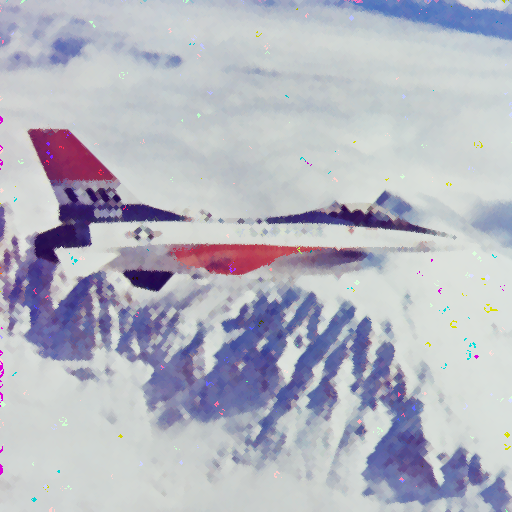
\includegraphics[width=0.9\linewidth]{../images/outputs/denoise/co/co5.png}
    
    \centering
  \end{subfigure}
 \caption{close-opening with proposed method}
 \end{subfigure}

  \begin{subfigure}{0.9\textwidth}
   \centering
\begin{subfigure}[t]{0.15\textwidth}
    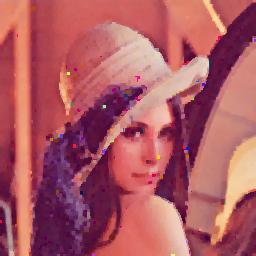
\includegraphics[width=0.9\linewidth]{../images/outputs/denoise/hg/hg0.png}
    
    \centering
  \end{subfigure}
\begin{subfigure}[t]{0.15\textwidth}
    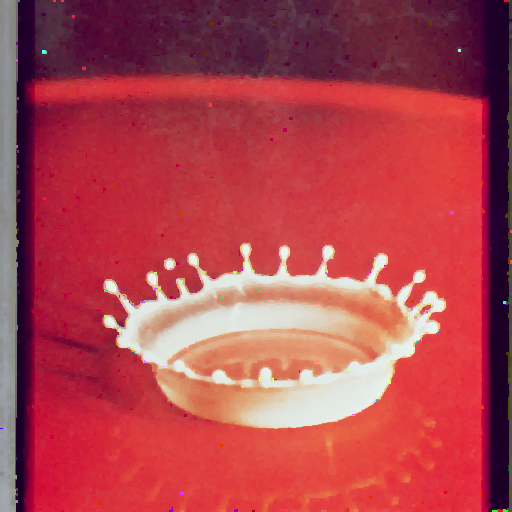
\includegraphics[width=0.9\linewidth]{../images/outputs/denoise/hg/hg1.png}
    
    \centering
  \end{subfigure}
\begin{subfigure}[t]{0.15\textwidth}
    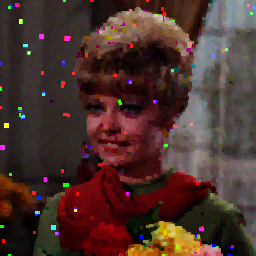
\includegraphics[width=0.9\linewidth]{../images/outputs/denoise/hg/hg2.png}
    
    \centering
  \end{subfigure}
\begin{subfigure}[t]{0.15\textwidth}
    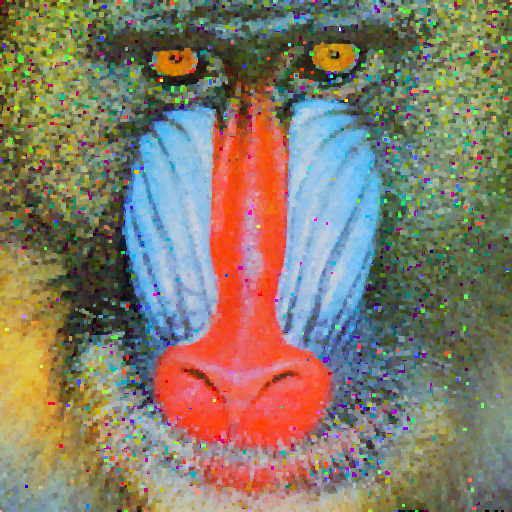
\includegraphics[width=0.9\linewidth]{../images/outputs/denoise/hg/hg3.png}
    
    \centering
  \end{subfigure}
\begin{subfigure}[t]{0.15\textwidth}
    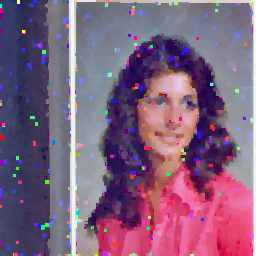
\includegraphics[width=0.9\linewidth]{../images/outputs/denoise/hg/hg4.png}
    
    \centering
  \end{subfigure}
\begin{subfigure}[t]{0.15\textwidth}
    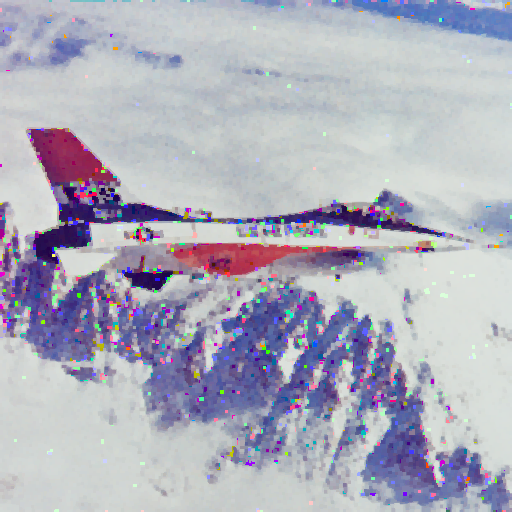
\includegraphics[width=0.9\linewidth]{../images/outputs/denoise/hg/hg5.png}
    
    \centering
  \end{subfigure}
 \caption{Wang's close-opening}
 \end{subfigure}

\end{figure}

% \begin{figure}[!ht]
   \centering
\begin{subfigure}[t]{0.22\textwidth}
    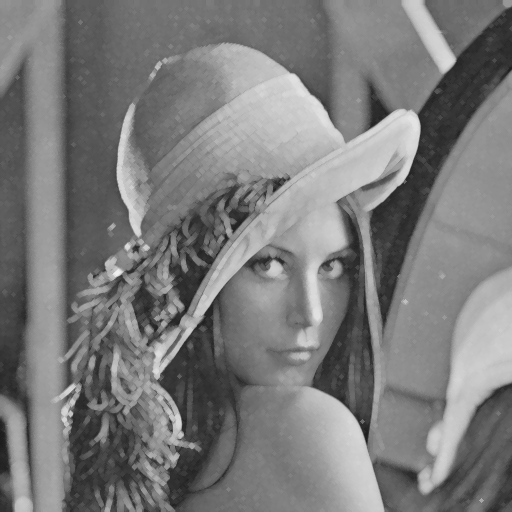
\includegraphics[width=0.9\linewidth]{../project/images/outputs/compare_gray/dilation.png}
    \caption{dilation, color}
    \centering
  \end{subfigure}
\begin{subfigure}[t]{0.22\textwidth}
    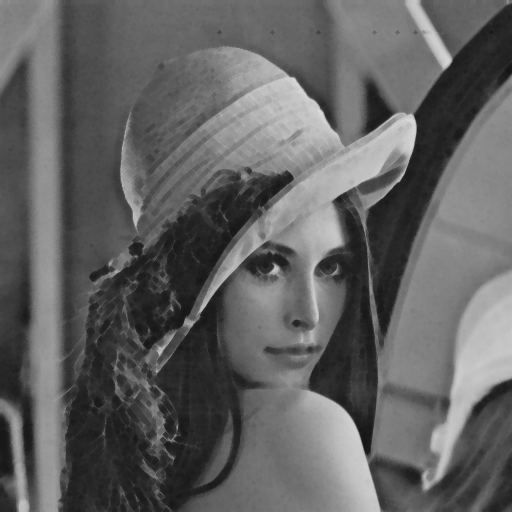
\includegraphics[width=0.9\linewidth]{../project/images/outputs/compare_gray/erosion.png}
    \caption{erosion, color}
    \centering
  \end{subfigure}
\begin{subfigure}[t]{0.22\textwidth}
    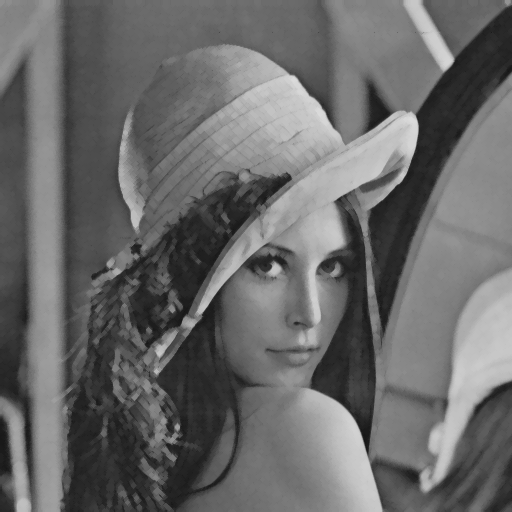
\includegraphics[width=0.9\linewidth]{../project/images/outputs/compare_gray/opening.png}
    \caption{opening, color}
    \centering
  \end{subfigure}
\begin{subfigure}[t]{0.22\textwidth}
    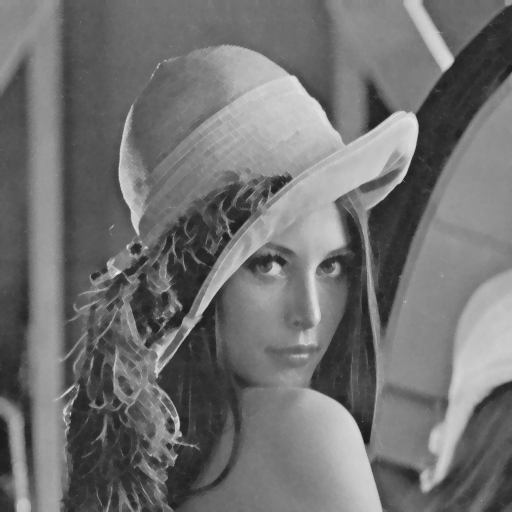
\includegraphics[width=0.9\linewidth]{../project/images/outputs/compare_gray/closing.png}
    \caption{closing, color}
    \centering
  \end{subfigure}
\begin{subfigure}[t]{0.22\textwidth}
    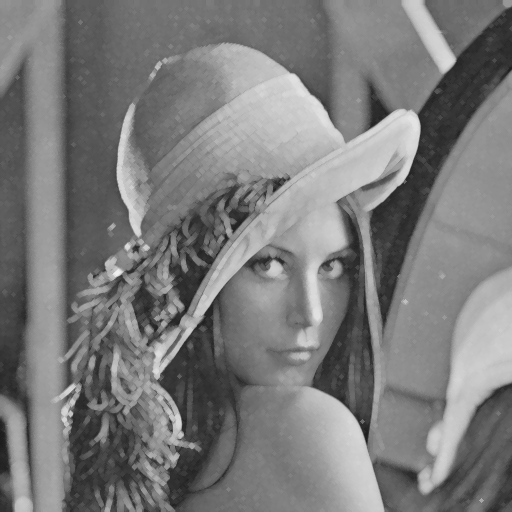
\includegraphics[width=0.9\linewidth]{../project/images/outputs/compare_gray/dilation_gray.png}
    \caption{dilation, gray}
    \centering
  \end{subfigure}
\begin{subfigure}[t]{0.22\textwidth}
    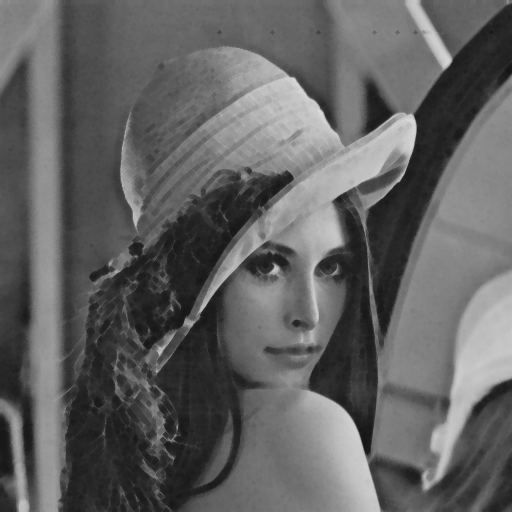
\includegraphics[width=0.9\linewidth]{../project/images/outputs/compare_gray/erosion_gray.png}
    \caption{erosion, gray}
    \centering
  \end{subfigure}
\begin{subfigure}[t]{0.22\textwidth}
    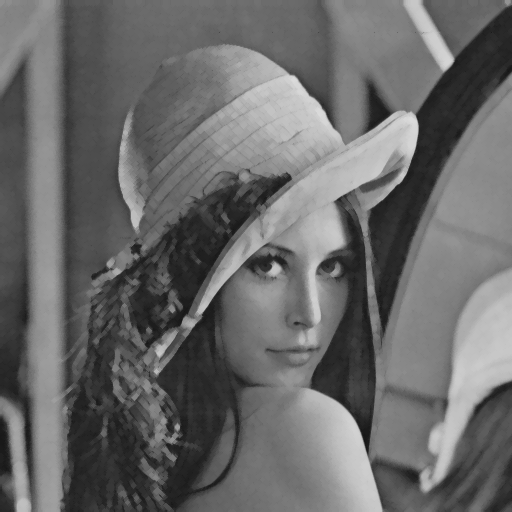
\includegraphics[width=0.9\linewidth]{../project/images/outputs/compare_gray/opening_gray.png}
    \caption{opening, gray}
    \centering
  \end{subfigure}
\begin{subfigure}[t]{0.22\textwidth}
    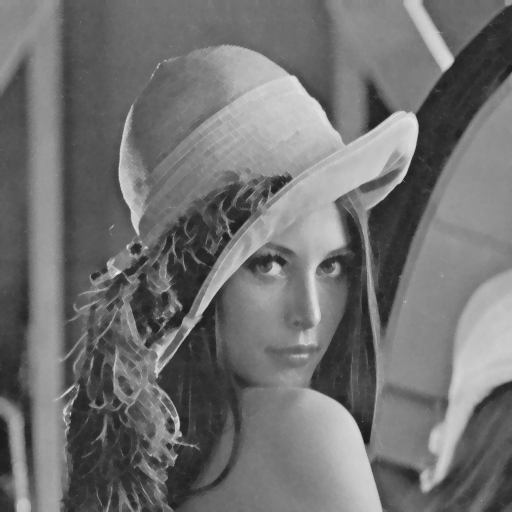
\includegraphics[width=0.9\linewidth]{../project/images/outputs/compare_gray/closing_gray.png}
    \caption{closing, gray}
    \centering
  \end{subfigure}
\begin{subfigure}[t]{0.22\textwidth}
    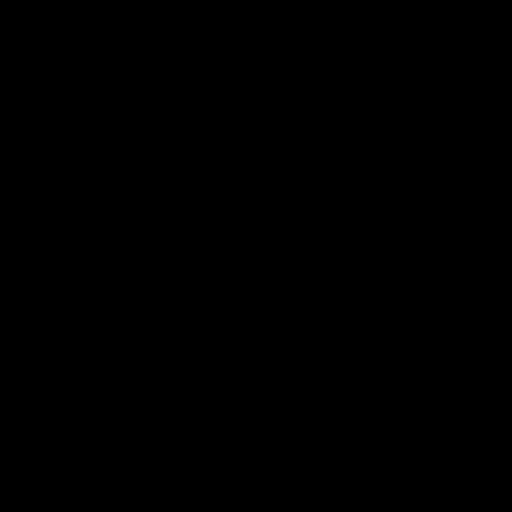
\includegraphics[width=0.9\linewidth]{../project/images/outputs/compare_gray/dilation_diff.png}
    \caption{dilation, diff}
    \centering
  \end{subfigure}
\begin{subfigure}[t]{0.22\textwidth}
    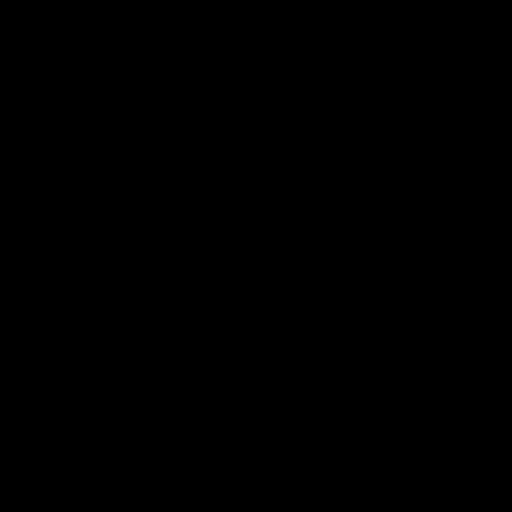
\includegraphics[width=0.9\linewidth]{../project/images/outputs/compare_gray/erosion_diff.png}
    \caption{erosion, diff}
    \centering
  \end{subfigure}
\begin{subfigure}[t]{0.22\textwidth}
    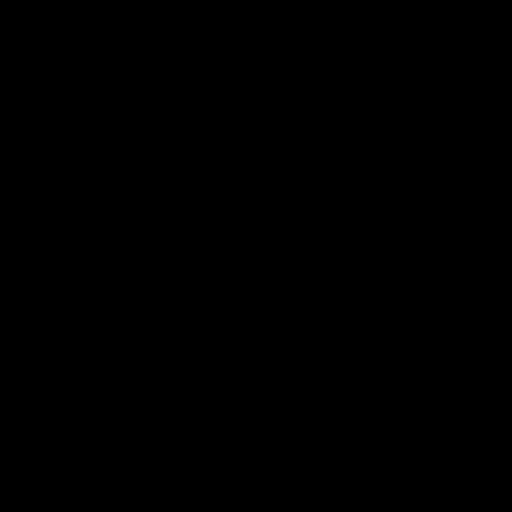
\includegraphics[width=0.9\linewidth]{../project/images/outputs/compare_gray/opening_diff.png}
    \caption{opening, diff}
    \centering
  \end{subfigure}
\begin{subfigure}[t]{0.22\textwidth}
    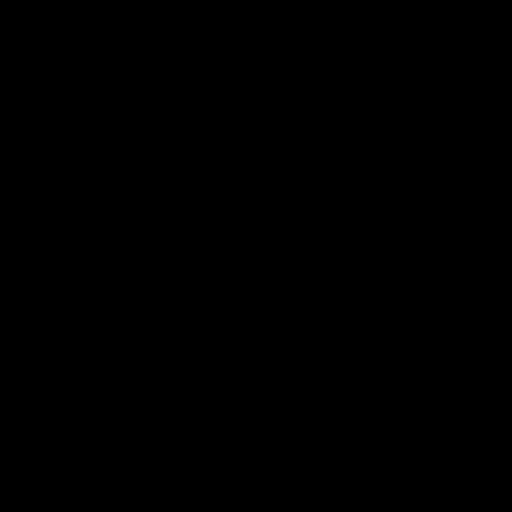
\includegraphics[width=0.9\linewidth]{../project/images/outputs/compare_gray/closing_diff.png}
    \caption{closing, diff}
    \centering
  \end{subfigure}
 \caption{}
 \end{figure}

% \begin{figure}[!ht]
   \centering
\begin{subfigure}[t]{0.22\textwidth}
    \includegraphics[width=0.9\linewidth]{../project/images/outputs/compare\_mode1/dilation\_sum.png}
    \caption{dilation with sum}
    \centering
  \end{subfigure}
\begin{subfigure}[t]{0.22\textwidth}
    \includegraphics[width=0.9\linewidth]{../project/images/outputs/compare\_mode1/erosion\_sum.png}
    \caption{erosion with sum}
    \centering
  \end{subfigure}
\begin{subfigure}[t]{0.22\textwidth}
    \includegraphics[width=0.9\linewidth]{../project/images/outputs/compare\_mode1/opening\_sum.png}
    \caption{opening with sum}
    \centering
  \end{subfigure}
\begin{subfigure}[t]{0.22\textwidth}
    \includegraphics[width=0.9\linewidth]{../project/images/outputs/compare\_mode1/closing\_sum.png}
    \caption{closing with sum}
    \centering
  \end{subfigure}
\begin{subfigure}[t]{0.22\textwidth}
    \includegraphics[width=0.9\linewidth]{../project/images/outputs/compare\_mode1/dilation\_prod.png}
    \caption{dilation with prod}
    \centering
  \end{subfigure}
\begin{subfigure}[t]{0.22\textwidth}
    \includegraphics[width=0.9\linewidth]{../project/images/outputs/compare\_mode1/erosion\_prod.png}
    \caption{erosion with prod}
    \centering
  \end{subfigure}
\begin{subfigure}[t]{0.22\textwidth}
    \includegraphics[width=0.9\linewidth]{../project/images/outputs/compare\_mode1/opening\_prod.png}
    \caption{opening with prod}
    \centering
  \end{subfigure}
\begin{subfigure}[t]{0.22\textwidth}
    \includegraphics[width=0.9\linewidth]{../project/images/outputs/compare\_mode1/closing\_prod.png}
    \caption{closing with prod}
    \centering
  \end{subfigure}
\begin{subfigure}[t]{0.22\textwidth}
    \includegraphics[width=0.9\linewidth]{../project/images/outputs/compare\_mode1/dilation\_median.png}
    \caption{dilation with median}
    \centering
  \end{subfigure}
\begin{subfigure}[t]{0.22\textwidth}
    \includegraphics[width=0.9\linewidth]{../project/images/outputs/compare\_mode1/erosion\_median.png}
    \caption{erosion with median}
    \centering
  \end{subfigure}
\begin{subfigure}[t]{0.22\textwidth}
    \includegraphics[width=0.9\linewidth]{../project/images/outputs/compare\_mode1/opening\_median.png}
    \caption{opening with median}
    \centering
  \end{subfigure}
\begin{subfigure}[t]{0.22\textwidth}
    \includegraphics[width=0.9\linewidth]{../project/images/outputs/compare\_mode1/closing\_median.png}
    \caption{closing with median}
    \centering
  \end{subfigure}
 \caption{}
 \end{figure}

% \begin{figure}[!ht]
   \centering
\begin{subfigure}[t]{0.22\textwidth}
    \includegraphics[width=0.9\linewidth]{../images/outputs/compare\_mode1/dilation\_sum.png}
    \caption{dilation with sum}
    \centering
  \end{subfigure}
\begin{subfigure}[t]{0.22\textwidth}
    \includegraphics[width=0.9\linewidth]{../images/outputs/compare\_mode1/erosion\_sum.png}
    \caption{erosion with sum}
    \centering
  \end{subfigure}
\begin{subfigure}[t]{0.22\textwidth}
    \includegraphics[width=0.9\linewidth]{../images/outputs/compare\_mode1/opening\_sum.png}
    \caption{opening with sum}
    \centering
  \end{subfigure}
\begin{subfigure}[t]{0.22\textwidth}
    \includegraphics[width=0.9\linewidth]{../images/outputs/compare\_mode1/closing\_sum.png}
    \caption{closing with sum}
    \centering
  \end{subfigure}
\begin{subfigure}[t]{0.22\textwidth}
    \includegraphics[width=0.9\linewidth]{../images/outputs/compare\_mode1/dilation\_prod.png}
    \caption{dilation with product}
    \centering
  \end{subfigure}
\begin{subfigure}[t]{0.22\textwidth}
    \includegraphics[width=0.9\linewidth]{../images/outputs/compare\_mode1/erosion\_prod.png}
    \caption{erosion with product}
    \centering
  \end{subfigure}
\begin{subfigure}[t]{0.22\textwidth}
    \includegraphics[width=0.9\linewidth]{../images/outputs/compare\_mode1/opening\_prod.png}
    \caption{opening with product}
    \centering
  \end{subfigure}
\begin{subfigure}[t]{0.22\textwidth}
    \includegraphics[width=0.9\linewidth]{../images/outputs/compare\_mode1/closing\_prod.png}
    \caption{closing with product}
    \centering
  \end{subfigure}
\begin{subfigure}[t]{0.22\textwidth}
    \includegraphics[width=0.9\linewidth]{../images/outputs/compare\_mode1/dilation\_median.png}
    \caption{dilation with median}
    \centering
  \end{subfigure}
\begin{subfigure}[t]{0.22\textwidth}
    \includegraphics[width=0.9\linewidth]{../images/outputs/compare\_mode1/erosion\_median.png}
    \caption{erosion with median}
    \centering
  \end{subfigure}
\begin{subfigure}[t]{0.22\textwidth}
    \includegraphics[width=0.9\linewidth]{../images/outputs/compare\_mode1/opening\_median.png}
    \caption{opening with median}
    \centering
  \end{subfigure}
\begin{subfigure}[t]{0.22\textwidth}
    \includegraphics[width=0.9\linewidth]{../images/outputs/compare\_mode1/closing\_median.png}
    \caption{closing with median}
    \centering
  \end{subfigure}
 \caption{Comparison of different modes}
 \end{figure}

% \begin{figure}[!ht]
  \centering
  \begin{subfigure}[t]{0.4\textwidth}
    \includegraphics[width=0.9\linewidth]{../images/outputs/compare\_global/imgs\_0.png}
    \caption{Local orders}
    \centering
  \end{subfigure}
  \begin{subfigure}[t]{0.4\textwidth}
    \includegraphics[width=0.9\linewidth]{../images/outputs/compare\_global/imgs\_1.png}
    \caption{Local orders (fuzzy)}
    \centering
  \end{subfigure}
  \begin{subfigure}[t]{0.4\textwidth}
    \includegraphics[width=0.9\linewidth]{../images/outputs/compare\_global/imgs\_2.png}
    \caption{Local orders (argsort)}
    \centering
  \end{subfigure}
  \begin{subfigure}[t]{0.4\textwidth}
    \includegraphics[width=0.9\linewidth]{../images/outputs/compare\_global/imgs\_3.png}
    \caption{Local orders (argsort, fuzzy)}
    \centering
  \end{subfigure}
  \begin{subfigure}[t]{0.4\textwidth}
    \includegraphics[width=0.9\linewidth]{../images/outputs/compare\_global/imgs\_4.png}
    \caption{Global orders}
    \centering
  \end{subfigure}
  \begin{subfigure}[t]{0.4\textwidth}
    \includegraphics[width=0.9\linewidth]{../images/outputs/compare\_global/imgs\_5.png}
    \caption{Global orders (fuzzy)}
    \centering
  \end{subfigure}
  \caption{Comparison of dilation with global and local orders}
\end{figure}

% \begin{figure}[!ht]
   \centering
\begin{subfigure}[t]{0.22\textwidth}
    \includegraphics[width=0.9\linewidth]{../images/outputs/compare\_order/dilation\_proposed.png}
    \caption{dilation with proposed}
    \centering
  \end{subfigure}
\begin{subfigure}[t]{0.22\textwidth}
    \includegraphics[width=0.9\linewidth]{../images/outputs/compare\_order/dilation\_proposed\_fuzzy.png}
    \caption{dilation with proposed (fuzzy)}
    \centering
  \end{subfigure}
\begin{subfigure}[t]{0.22\textwidth}
    \includegraphics[width=0.9\linewidth]{../images/outputs/compare\_order/erosion\_proposed.png}
    \caption{erosion with proposed}
    \centering
  \end{subfigure}
\begin{subfigure}[t]{0.22\textwidth}
    \includegraphics[width=0.9\linewidth]{../images/outputs/compare\_order/erosion\_proposed\_fuzzy.png}
    \caption{erosion with proposed (fuzzy)}
    \centering
  \end{subfigure}
\begin{subfigure}[t]{0.22\textwidth}
    \includegraphics[width=0.9\linewidth]{../images/outputs/compare\_order/dilation\_HSV.png}
    \caption{dilation with HSV}
    \centering
  \end{subfigure}
\begin{subfigure}[t]{0.22\textwidth}
    \includegraphics[width=0.9\linewidth]{../images/outputs/compare\_order/dilation\_HSV\_fuzzy.png}
    \caption{dilation with HSV (fuzzy)}
    \centering
  \end{subfigure}
\begin{subfigure}[t]{0.22\textwidth}
    \includegraphics[width=0.9\linewidth]{../images/outputs/compare\_order/erosion\_HSV.png}
    \caption{erosion with HSV}
    \centering
  \end{subfigure}
\begin{subfigure}[t]{0.22\textwidth}
    \includegraphics[width=0.9\linewidth]{../images/outputs/compare\_order/erosion\_HSV\_fuzzy.png}
    \caption{erosion with HSV (fuzzy)}
    \centering
  \end{subfigure}
\begin{subfigure}[t]{0.22\textwidth}
    \includegraphics[width=0.9\linewidth]{../images/outputs/compare\_order/dilation\_gray scale.png}
    \caption{dilation with gray scale}
    \centering
  \end{subfigure}
\begin{subfigure}[t]{0.22\textwidth}
    \includegraphics[width=0.9\linewidth]{../images/outputs/compare\_order/dilation\_gray scale\_fuzzy.png}
    \caption{dilation with gray scale (fuzzy)}
    \centering
  \end{subfigure}
\begin{subfigure}[t]{0.22\textwidth}
    \includegraphics[width=0.9\linewidth]{../images/outputs/compare\_order/erosion\_gray scale.png}
    \caption{erosion with gray scale}
    \centering
  \end{subfigure}
\begin{subfigure}[t]{0.22\textwidth}
    \includegraphics[width=0.9\linewidth]{../images/outputs/compare\_order/erosion\_gray scale\_fuzzy.png}
    \caption{erosion with gray scale (fuzzy)}
    \centering
  \end{subfigure}
 \caption{Comparison of RGB and HSV orderings}
 \end{figure}





\end{document}